\subsection{SSC Black Witch}

\begin{center}
    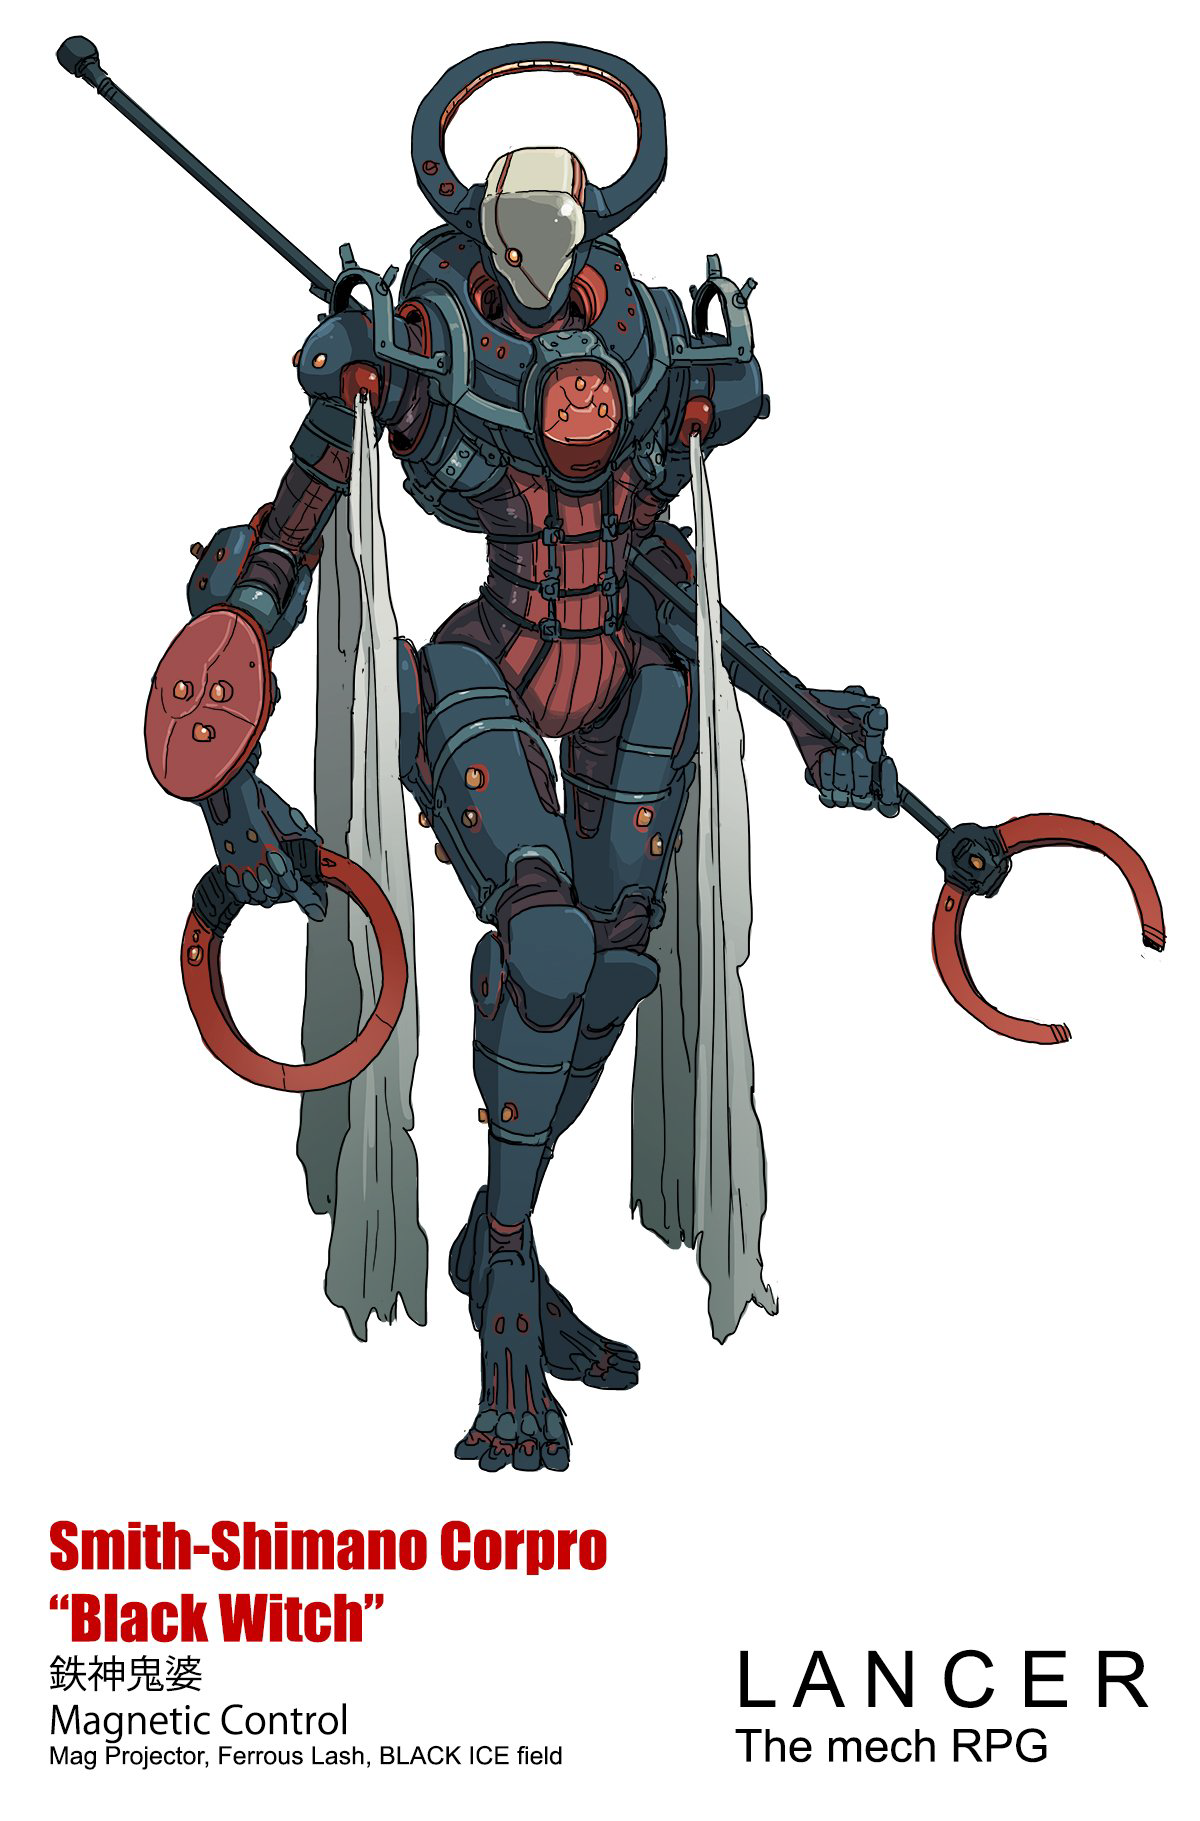
\includegraphics{BlackWitch}
\end{center}

\begin{mech}{SSC}{Black Witch}

\fluff{The BLACK WITCH is the primary designate model in SSC's newest line of mech cores meant to compete with HORUS's dominance in the field of invasion/control cores. The BLACK WITCH is open to all pilots with the necessary SSC licensing and should experience greater overall use, as current SSC licenses outnumber the hypothetical maximum of HORUS licenses issued. The BLACK WITCH is built to withstand the stresses of combat system invasion and magnetic weaponry: it is a primary platform for engagements where the use of kinetic, ferrous projectiles and ordinance is expected. Developed primarily as a salvage and scrap repair system, the SSC-BW's mag field system was soon repurposed by the SSC Gendarme as a personal defense system}

\begin{license}
\item Ferrous Lash, Mag Cannon
\item BLACK WITCH FRAME, ICE-OUT Drone, Mag Deployer
\item Black ICE module, Mag Shield
\end{license}

\frameBox
[hp = 6,
evasion = 10,
speed = 5,
heat cap = 6,
sensors = 15,
armor = 1,
e-defense = 12,
size = 1,
repair cap = 3,
tech attack = +1,
traits = {\textbf{Repulsor field:} The Black witch is resistant to kinetic damage

\textbf{Mag parry:} 1/round you can attempt to parry any attack that deals kinetic damage against you or an adjacent ally as a reaction. Roll a d6. On a 5+, the attack is negated and automatically misses.},
sp = 8,
mount one = aux/aux mount,
mount two = main mount,
core system name = Mag Projector,
core system text = {A magnetic field generator takes the same technology as other projected magnetic defenses and makes them portable separate from a mech core. When activated, the mag field generator creates a projected magnetic bubble that traps all incoming ferrous projectiles; the strength of the field is so great that it can even draw mechs to its center. When the field is canceled or the solid-state battery burns out (by design), the field detonates through sudden catastrophic reversal, launching all captured projectiles out from its center.},
core active name = Mag Field,
core active text = {As a quick action, you may activate the mag field to create a Blast 4 area in any area with at least one square adjacent to you. Inside, ranged weapon attacks that deal kinetic or explosive damage cannot penetrate into or out of the field and will stop at the edge, doing no damage (keep track of them). The field is difficult terrain for all mechs and vehicles made at least partly of metal. Actors at least partly made of metal that start their turn in the Mag Field or enter it for the first time on their turns must make a successful Engineering check with 1 difficulty or be pulled to the center as far as possible and immobilized. They can repeat this check at the start of their subsequent turns while trapped this way and can move normally on a success, otherwise they remain trapped. The field lasts until the end of your next turn. At the end of your next turn, any kinetic or explosive weapons fired into this field will resume trajectory towards the center of this zone. The GM performs a single attack roll vs each target still inside the zone with +1 targeting per attack fired into this zone (cumulative, up to a max of +6). Successful hits deal 1d6 Kinetic damage per attack fired into this zone (cumulative, to a maximum of 6d6). Then, the zone deactivates.}]


Mag Cannon

The SSC Magnetic Cannon is a first in Smith-Shimano's ENERGY line: an aperture-focused magnetic projection beam that disrupts and damages hardware using intense pulses of magnetic force. Cores caught in the beam of a mag cannon suffer additional damage to their software, as even hardened components come under massive systemic stress.

Main Cannon

1 heat (self)
Line 8
1d3 energy damage +1 heat

All targets caught in the area of this weapon must pass a systems check or become impaired until the end of their next turn.


Ferrous Lash

Initially developed as a non lethal crowd suppression device, the Ferrous Lash is a far more complex and dangerous device in the right pilot's hands. Fired from a series of integrated launchers, the FL system detonates payloads of fast-congeal ferrofluids that restrain their targets; tuned to the correct frequency, these proprietary SSC ferrofluid blends form into rudimentary ambulatory segments, pulling their hosts back towards the casting unit.

2 SP
Quick Action

A target of your choice in range 10 must pass an agility check with 1 difficulty. On a failure, it is knocked back 5 in a direction of your choice. This movement must obey obstructions, terrain, etc, but doesn't provoke reactions and ignores engagement. If it collides with an obstacle or another mech, it is additionally knocked prone.


ICEOUT drone

SSC's ICEOUT module is a response to the increasing reliance on system-based scans to ensure accurate targeting. By blanketing a core's systems in layers of digital defilade, mirroring, spoofing, and redirection, an ICEOUT module can effectively disappear/disincorporate/legion its user from hostile scans. Note that this module only makes its user system-invisible; they will still be visible through optics.

2 SP, Limited (2)
Drone, quick action

You fire an ICEOUT drone at a point within range 10 of you, where it hovers in place. The drone is invisible. Once fired, the drone creates a burst 2 zone around itself. Any target at least partially covered by the zone, allied or enemy, is immune to all tech actions (even beneficial ones), and cannot make or benefit from any tech actions. Any negative statuses caused by tech actions immediately end. Targets inside the zone don't show up on any electronic sensors and are only visible to the naked eye or optics. The drone deactivates at the end of the current scene or when destroyed, and cannot be re-used. You can move it again to a point in your sensor range as a quick action.


Mag Deployer
SSC's own take on flash-printing is advanced enough to embed magtech burnout cells into raw prefab clay. SSC non-mag pilots often disparage Black Witch pilots for ``throwing plates'' at the enemy, but the tactical advantage they provide cannot be denied.

2 SP
Quick action.

You flash-print a heavy metal plate that takes up a 2x2 free space in range 5 of you. It is flat and doesn't obstruct movement. You can set the system to one of two settings when you create it:

         Repulse: Any hostile target that enters the space must pass a hull check or be pushed in a direction of your choice 3 spaces. If this causes them to collide with an obstruction (terrain, a mech, etc) it is additionally knocked prone. An allied target that enters the space can fly 3 in any direction as a free action.

         Attract: Any target, allied or enemy, that enters the space, must pass a hull check or become immobilized. It can end this status by taking a quick action and repeating this check successfully to free itself.

The deployer can be attacked - it has evasion 5, 20 hp, and 2 armor, and it lasts until the end of the current challenge or around an hour outside. You can only deploy one at at time. If you create a new deployer, the old one disintegrates and is destroyed.


Black Ice module

3 SP, Unique

Hostile tech actions or system attacks against your mech or any adjacent ally are made at +1 Difficulty. Successive attacks in the same combat from any target are made with an additional +1 Difficulty (cumulative). This difficulty has a maximum of +4, and resets when it would hit +5 back to +1 as its definitions roll over.


Mag Shield
SSC's magnetic shield takes the same technology as their proprietary magnetic buckler and applies it to a massive deployable system.

2 SP, Unique
Shield, quick action

As a quick action, this system creates a line 4 force field 4 spaces high with at least 1 square in an adjacent space to you. Any adjacent mech can use this force field for heavy cover from attacks on the other side. It additionally gains resistance to kinetic and explosive damage from attacks on the other side of this field, but conversely, any of its targets on the other side of the forcefield gain resistance to kinetic and explosive damage from its attacks. The shield lasts until the end of the current scene, but only 1 shield can be placed at a time.
\end{mech}
